\documentclass[english]{jflart}
\usepackage[utf8]{inputenc}
\usepackage[T1]{fontenc}
\usepackage{minted}
\usepackage{etoolbox,xpatch}
\usepackage{ tipa }
\usepackage{float}
\usepackage[normalem]{ulem}
\usepackage[backend=biber, style=alphabetic]{biblatex}
\usepackage{newunicodechar}
\usepackage[section]{placeins}
\addbibresource{bibliography.bib}

% Numéro et année des JFLAs visées par l'article, obligatoire.
\jfla{35}{2024}

\title{Destination-passing style programming: a Haskell implementation}
% Un titre plus court, optionnel.
%\titlerunning{Du bon usage de~\texttt{jflart.cls}}

% Auteurs, liste non abrégée.
\author[1]{Thomas Bagrel}
% \author[2]{Cunégonde Martin}
% \author[2]{Odoacre Contempierre}
% Une liste d'auteurs abrégée à utiliser à l'intérieur de l'article.
\authorrunning{Bagrel}

% Affiliations des auteurs
\affil[1]{INRIA/LORIA, Vand\oe{}uvre-lès-Nancy, 54500, France}
\affil[2]{TWEAG, Paris, 75012, France}

% Une commande définie par l'utilisateur
\newcommand{\cmd}[1]{\texttt{\textbackslash {#1}}}
\newcommand{\mpar}{\text{\,\textramshorns\,}}
\newcommand{\dest}{-\prec}
\newcommand{\TODO}[1]{{\color{red}\large #1}}
\newcommand{\mnew}[1]{\colorbox{green}{#1}}
\newcommand{\muline}[1]{\uline{#1}}
\newcommand{\mold}[1]{\colorbox{red}{#1}}
\newunicodechar{⊸}{\ensuremath{\multimap}}
\newunicodechar{→}{\ensuremath{\to}}
\newunicodechar{⇒}{\ensuremath{\Rightarrow}}
\newunicodechar{;}{\textbf{\large;}}
\newunicodechar{∀}{\ensuremath{\forall}}
\makeatletter
\AtBeginEnvironment{minted}{\dontdofcolorbox}
\def\dontdofcolorbox{\renewcommand\fcolorbox[4][]{##4}}
\xpatchcmd{\inputminted}{\minted@fvset}{\minted@fvset\dontdofcolorbox}{}{}
\xpatchcmd{\mintinline}{\minted@fvset}{\minted@fvset\dontdofcolorbox}{}{} % see https://tex.stackexchange.com/a/401250/
\makeatother

\begin{document}

\maketitle

\begin{abstract}
Destination-passing style programming introduces destinations, which represents the address of a write-once memory cell. Those destinations can be passed around as function parameters, and thus enable the caller of a function to keep control over memory allocation: the body of the called function will just be responsible of filling that memory cell. This is especially useful in functional programming languages such as Haskell, in which the body of a function is typically responsible for allocation of the result value.

Programming with destination in Haskell is an interesting way to improve performance of critical parts of some programs, without sacrificing memory warranties. Indeed, thanks to a linearly-typed API we designed, a write-once memory cell cannot be left uninitialized before being read, and is still disposed of by the garbage collector when it is not in use anymore, eliminating the risk of uninitialized read, memory leak, or double-free errors that can arise when memory is handled manually.

With the implementation of destinations for Haskell through compact regions we provide in this article, we reach a 15-40\% improvement over memory allocation in a simple parser example, and 0-50\% improvement in run time. We also provide a few examples of programs that can be implemented in a tail-recursive fashion thanks to destinations, which is crucial for performance in strict contexts.

Safety proofs for the API are not provided in this article though, and will be the subject of a future article.
\end{abstract}

\tableofcontents{}

\section{Introduction}

% TODO: Linear constraints

Destinations bring a taste of imperative programming in a pure functional environnement when performance really matters, without breaking memory safety.

Using destinations as a way of allocating and building functional data structures can lead to better time and/or space performance for critical parts of a program, but destinations also increase expressiveness of a functional language.

\TODO{Write introduction}

%TODO: conceptuellement simple, mais beaucoup d'obstacles techniques pour rendre ça possible.
% TODO GHC where purity is enforced
% TODO Also because it has good support for linear type discipline
% TODO Linear types
% TODO Destinations
% TODO Compact regions
% TODO strict lazy haskell
% TODO <&>

\section{Motivating examples for destination-passing style programming}\label{sec:motivating-examples}

Destination-passing style (DPS) programming takes its source in the early days of imperative languages with manual memory management. In the C programming language, it's quite common for a function not to allocate memory itself for its result, but rather to receive a reference to a memory location where to write its result (often named \emph{out(put) parameter}). In that scheme, the caller of the function is both responsible for allocation and disposal of the cell in which the value will live. This is exactly what DPS programming is about: take control from the callee back to the caller about memory management.

DPS programming needs a concept of reference or pointer to communicate the location of the memory cell in which the called function should write its result. In functional programming languages, these are often named \emph{destinations}, so we will use this name to refer to the address of a write-once memory cell in Haskell.

It's time to see why DPS programming can be useful even in a pure functional context such as Haskell.

\subsection{Efficient difference lists}

Linked lists are a staple of functional programming, but they aren't efficient for concatenation, especially when the concatenation calls are nested to the left.

In an imperative context, it would be quite easy to concatenate linked lists efficiently. One just have to keep both a pointer to the root and to the last \emph{cons} cell of each list. Then, to concatenate two lists, one just have to mutate the last \emph{cons} cell of the first one to point to the root of the second list.

It isn't possible to do so in an immutable functional context though. Instead, \emph{Difference lists} can be used: they are structures that are fast to convert into lists ($\mathcal{O}(1)$ amortized) and tend to emulate the idea of having a mutable (here, write-once) last \emph{cons} cell. Usually, a difference list \mintinline{haskell}`[x1, ..., xn, ?]` is encoded by a function taking a last element \mintinline{haskell}`ys` of type \mintinline{haskell}`[a]` and returning \mintinline{haskell}`x1 : ... : xn : ys` (having type \mintinline{haskell}`[a]` too). \TODO{reference for difference list paper}

With such representation, concatenation is just function composition: \mintinline{haskell}`f1 <> f2 = f1 . f2`, and we have \mintinline{haskell}`mempty = id`\footnote{\mintinline{haskell}`mempty` and \mintinline{haskell}`<>` are the standard notations for the neutral element and internal operation of a monoid in Haskell}, \mintinline{haskell}`toList f = f []` and \mintinline{haskell}`fromList xs = \ys → xs ++ xs`.

In DPS, instead of encoding the concept of a write-once hole with a function, we can represent the hole as a first-class object with a \emph{destination}. A difference list now become an actual data structure in memory --- not just a pending computation --- that has two handles: one to the root of the list of type \mintinline{haskell}`[a]`, and one to the yet-to-be-filled hole in the last cons cell, represented by a destination of type \mintinline{haskell}`Dest [a]`.

With the function encoding, it isn't possible to read the list until a last element of type \mintinline{haskell}`[a]` have been supplied to complete it. With the destination representation, this constraint must persists: the actual list \mintinline{haskell}`[a]` shouldn't be readable until the accompanying destination is filled (or \emph{linearly consumed}, as we sometimes write), otherwise memory safety wouldn't be respected. This constraint is embodied by the \mintinline{haskell}`Incomplete a b` type of our destination API: \mintinline{haskell}`b` is what needs to be linearly consumed to make the \mintinline{haskell}`a` readable. Most of the time, the \mintinline{haskell}`b` side carries the destinations of the structure. A difference list is then \mintinline{haskell}`type DList a = Incomplete [a] (Dest [a])`: one should fill the \mintinline{haskell}`Dest [a]` (with a \mintinline{haskell}`[a]`) to get a readable \mintinline{haskell}`[a]`.

% TODO
% How to fill these holes?

% 1. fillLeaf + schema
% 2. fill @' + schema
% 3. fillComp + schema
% Those 3 will be useful for the implementation of ...

The implementation of operations on destination-backed difference lists are presented in table~\ref{table:impl-dlist}.
\begin{table}[t]
\small
\begin{minted}[frame=single,framesep=10pt,linenos]{haskell}
data [a] -- built-in
  = []        -- nil constructor
  | (:) a [a] -- cons constructor

type DList a = Incomplete [a] (Dest [a])

alloc :: DList a

append :: DList a ⊸ a → DList a
append i x =
  i <&> \d → case fill @'(:) d of
    (dh, dt) → fillLeaf x dh ;; dt

concat :: DList a ⊸ DList a ⊸ DList a
concat i1 i2 = i1 <&> \dt1 -> fillComp i2 dt1

toList :: DList a ⊸ [a]
toList i = fromIncomplete_' (i <&> \dt → fill @'[] dt)
\end{minted}
\caption{Implementation of difference lists with destinations}
\label{table:impl-dlist}
\end{table}

\begin{figure}[t]
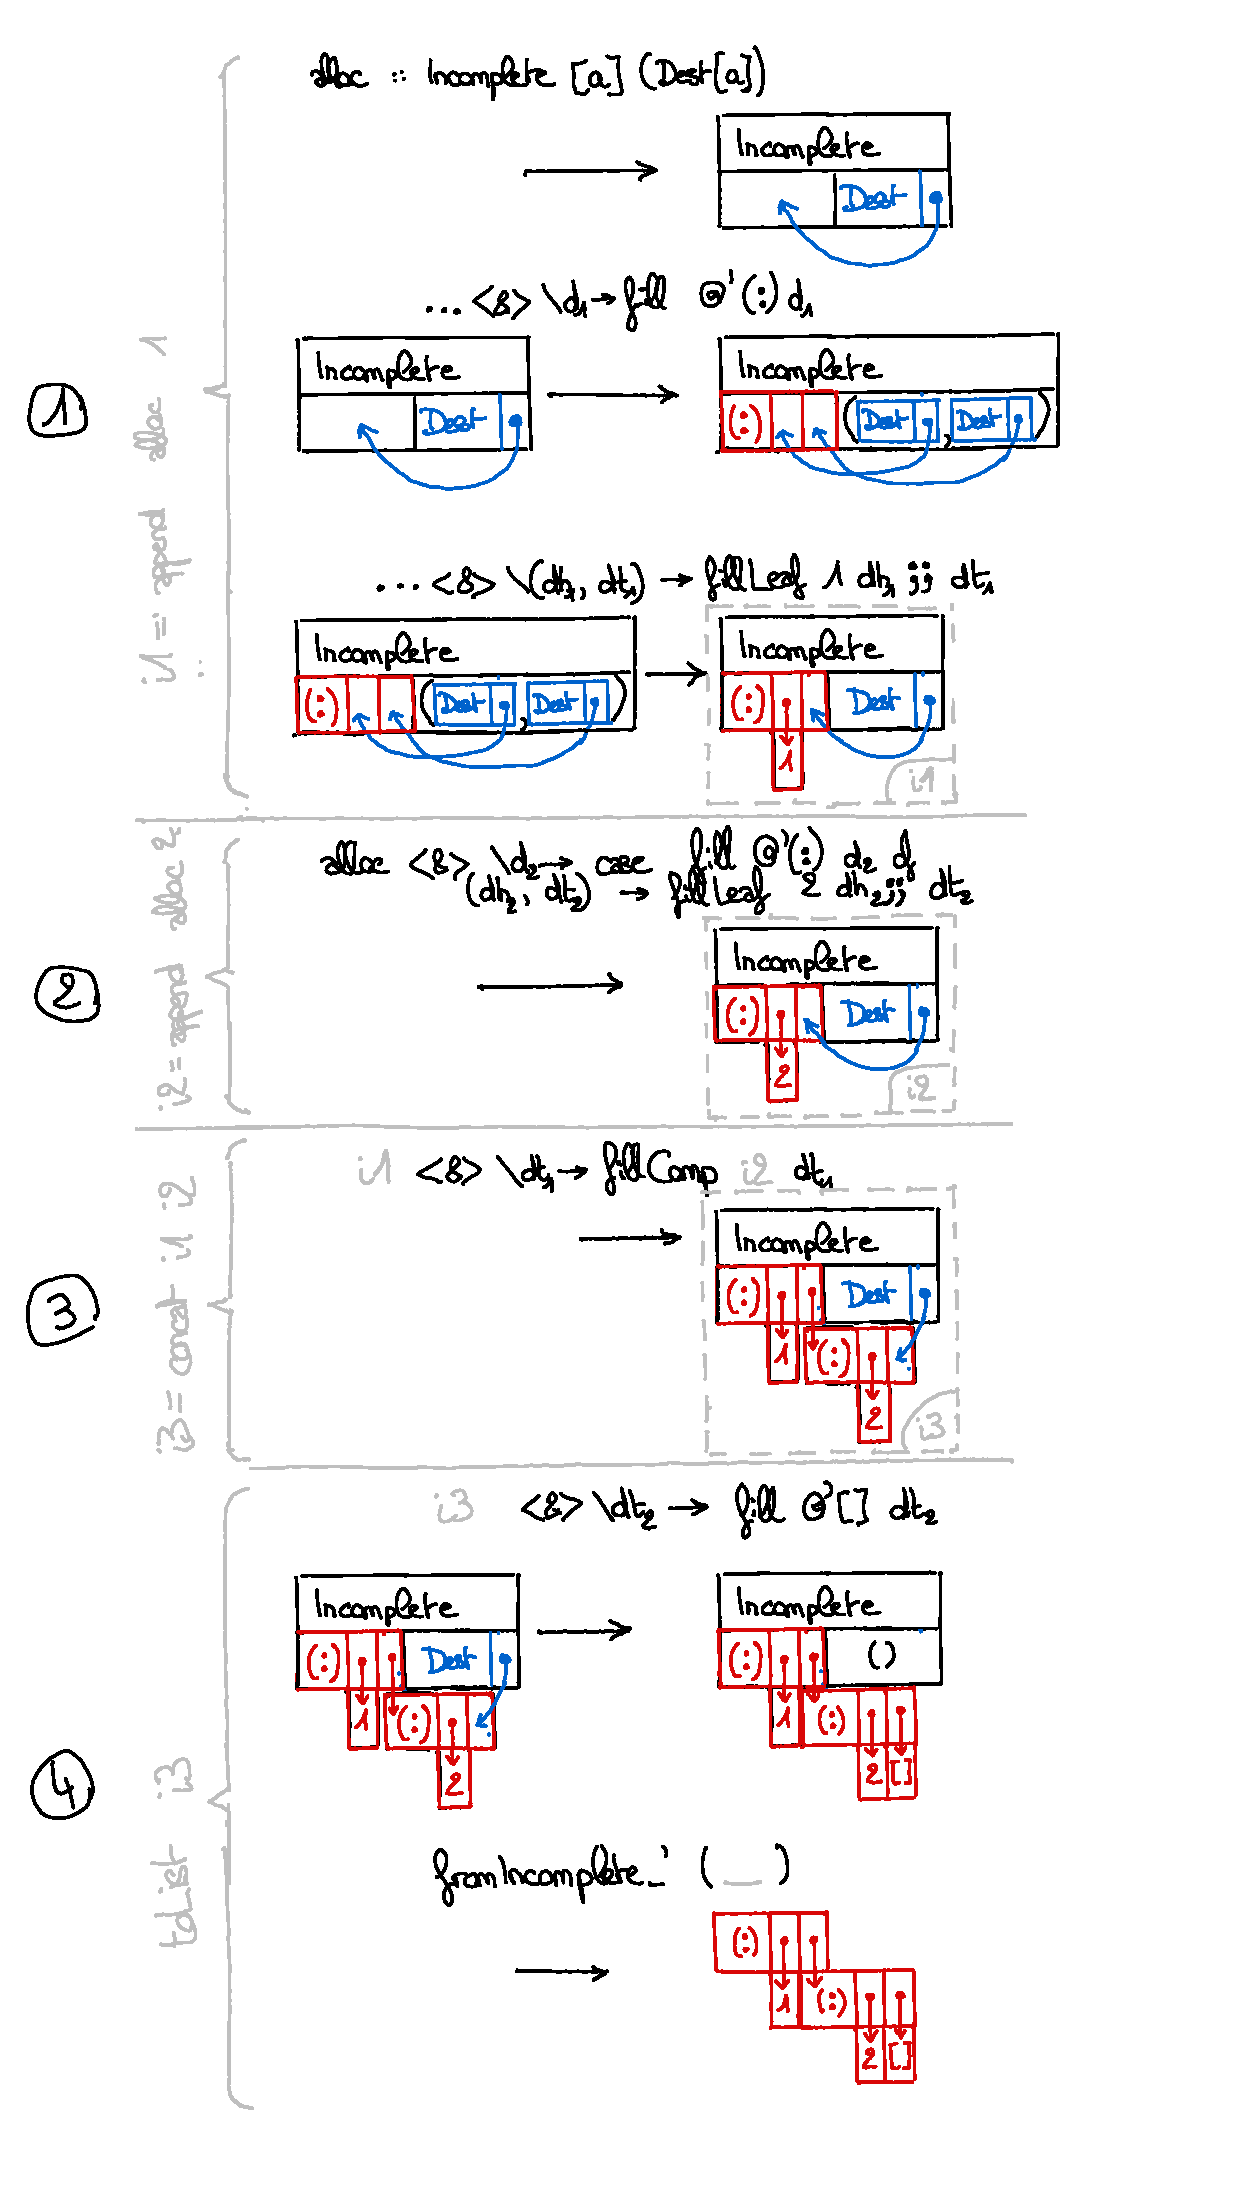
\includegraphics[height=22cm]{schema-dlist.pdf}
\caption{Memory behavior of difference lists backed by destinations}
\label{fig:schema-dlist}
\end{figure}

\begin{itemize}
  \item \mintinline{haskell}`alloc` returns a \mintinline{haskell}`DList a` which is exactly an \mintinline{haskell}`Incomplete [a] (Dest [a])` structure as shown at the top of part 1 of figure~\ref{fig:schema-dlist}. There is no data there yet; so the list that will be fed in the \mintinline{haskell}`Dest [a]` is exactly the list in that the \mintinline{haskell}`Incomplete` will hold. This is highly similar to the \mintinline{haskell}`id` function which represents the empty destination list in the function encoding;
  \item \mintinline{haskell}`append` fills the the hole at the end of the list \mintinline{haskell}`dl` with a new \emph{cons} cell, using \mintinline{haskell}`fill @'(:)`. The head of that cell \mintinline{haskell}`dh` is filled with the value to append using \mintinline{haskell}`fillLeaf`, and the remaining hole of the new \emph{cons} cell, represented by \mintinline{haskell}`dt :: Dest [a]`, is the hole of the resulting difference list, as shown in part 2 of figure~\ref{fig:schema-dlist};
  \item \mintinline{haskell}`concat` calls \mintinline{haskell}`fillComp`, which fills the destination of the first difference list \mintinline{haskell}`i1` with the root of the second difference list\mintinline{haskell}`i2`. The resulting \mintinline{haskell}`Incomplete` object hence has the same root as the first list, holds the elements of both lists, and has the hole of the second list at the end, as one can see in part 3 of figure~\ref{fig:schema-dlist}. Memory-wise, \mintinline{haskell}`concat` will just write the address of the root of the second list into the hole of the first one; no move is required.
  \item \mintinline{haskell}`toList` completes the incomplete structure by plugging \emph{nil} into its hole with \mintinline{haskell}`fill @'[]` and removes the \mintinline{haskell}`Incomplete` wrapper which is no longer useful, as shown in part 4 of figure~\ref{fig:schema-dlist}.
\end{itemize}

This simplified API for difference lists still lacks some linearity requirements to make it write-once/immutable. In particular, the result of \mintinline{haskell}`alloc` should be used linearly but this isn't enforced by this API, and as a result, one could fill the embedded destination twice. Linearity concerns will be addressed in Section~\ref{ssec:api-linearity}.

That being said, thanks to destination-style programming, not only we can express programs and functions whose implementation is closer to their intended memory behaviour (here, implementing data structures with holes), but we can also get important performance improvements too. \TODO{one sentence about the benchmark results compared to the function encoding}
\TODO{There should be an explanation in this section about why destinations have linearity requirement}

\TODO{remove clearpage}
\clearpage{}

\subsection{Breadth-first tree traversal}\label{ssec:bf-tree-traversal}

The idea of functional data structure with write-once holes is not new. In 1998, Minamide already proposed in~\cite{minamide_functional_1998} a variant of $\lambda$-calculus with support for \emph{hole abstractions}, which can be represented in memory by an incomplete structure with one hole and can be composed efficiently with each other (as with \mintinline{haskell}`fillComp` above). With such framework, it is fully possible to implement destination-backed difference lists, as we developed in the previous section.

However, in Minamide's work, there is no concept of destination: the hole in a structure can only be filled if one has the structure itself at hand. On the other hand, our paper introduces destinations, which are a way to interact with a hole remotely, even when one doesn't have a handle to the associated data structure. Because destination are treated as first-class objects, they can be passed around or stored in collections or other structure. Being able not only to represent data structures with holes, but also manipulate references to these holes as first-class objects while preserving memory safety, is the major step forward that this paper presents.

The fact that destinations can be stored in arbitrary data structures opens the way for more natural and efficient implementations of some functional data structure algorithms, for example breadth-first tree traversal, which isn't easy to implement in a standard immutable setting.

Consider the problem, which Okasaki attributes to Launchbury \TODO{Cite https://doi.org/10.1145/351240.351253}
\begin{quote}
  Given a tree $T$ , create a new tree of the same
  shape, but with the values at the nodes replaced
  by the numbers $1\ldots|T|$ in breadth-first order.
\end{quote}

This problem admits a straightforward implementation if we're allowed to mutate trees. But a pure implementation is quite tricky: it's the entire subject of Okasaki's paper \TODO{Cite https://doi.org/10.1145/351240.351253} as well as the earlier\TODO{Cite http://www.cs.ox.ac.uk/publications/publication2363-abstract.html}. More recently, a very elegant, albeit very clever, solution was proposed~\cite{gibbons_phases_2023}.

With storable destinations in our toolbelt, we can implement a solution that is both easy to come up with and efficient, doing only a single traversal pass on the original tree. The main idea is to keep a queue of pairs of a tree to be relabeled and the destination where the the relabeled result is expected (this is where destinations are stored!). Destinations make it possible to leave some parts of the tree ``unfinished'' for some time, and to come back to them later when it's their turn to be processed. The implementation provided in table~\ref{table:impl-bfs-tree-traversal}, really implements the slightly more general \mintinline{haskell}`mapAccumBFS`, which traverses a tree in breadth-first order and applies a relabeling function that can depend on a state.

\begin{table}[t]
\small
\begin{minted}[frame=single,framesep=10pt,linenos]{haskell}
data Tree a = Nil | Node a (Tree a) (Tree a)

relabelBFS :: Tree a → Tree Int
relabelBFS tree = fst (mapAccumBFS (\s _ -> (s+1, s)) 1 tree)

mapAccumBFS :: ∀ a b s. (s → a → (s, b)) → s → Tree a → (Tree b, s)
mapAccumBFS f s0 tree =
  fromIncomplete' (
    alloc <&> \dtree → go s0 (singleton (Ur tree, dtree)))
  where
    go :: s → Queue (Ur (Tree a), Dest (Tree b)) ⊸ Ur s
    go s q = case dequeue q of
      Nothing → Ur s
      Just ((utree, dtree), q') → case utree of
        Ur Nil → fill @'Nil dtree ;; go s q'
        Ur (Node x tl tr) → case fill @'Node dtree of
          (dr, dtl, dtr) →
            let q'' = q' `enqueue` (Ur tl, dtl) `enqueue` (Ur tr, dtr)
                (s', r) = f s x
              in fillLeaf r dr ;; go s' q''
\end{minted}
\caption{Implementation of breadth-first tree traversal with destinations}
\label{table:impl-bfs-tree-traversal}
\end{table}

Note that the signature of \mintinline{haskell}`mapAccumBFS` doesn't involve linear types. Linear types only appear in the inner loop \mintinline{haskell}`go`, which manipulates destinations. Linearity enforces the fact that every destination ever put in the queue is eventually filled at some point, which guarantees that the output tree is complete after the function has run, and thus can be made readable.

\TODO{Revisit the two paragraphs on Ur, below, when we have an introduction}
Because the state-transforming function \mintinline{haskell}`s → a → (s, b)` is non-linear, the leaves of the original tree (that are stored together with destinations in the queue) won't be consumed in a linear fashion. However, as we said, destinations must be all consumed linearly, and for that to hold, their container must be consumed linearly too. So we need a trick to indicate that one sub-part of the queue is allowed to be consumed non-linearly while the rest of the structure will appeared to be consumed linearly.

This is exactly the role that the \mintinline{haskell}`Ur` wrapper plays. A \mintinline{haskell}`Ur a` will appear to be consumed linearly even if its inner value of type \mintinline{haskell}`a` is consumed non-linearly. But only values coming from a non-linear source can be put wrapped in \mintinline{haskell}`Ur`. More precisely, \mintinline{haskell}`Ur` delimitates areas for non-linear values inside structures that are meant to be handled linearly, and only values already wrapped in \mintinline{haskell}`Ur` or coming from the left of a non-linear function arrow \mintinline{haskell}`→` can be put in another \mintinline{haskell}`Ur`. Destinations always appear on the left of linear function arrows \mintinline{haskell}`⊸`, so they couldn't be wrapped in \mintinline{haskell}`Ur` in an attempt to escape the API safety.

With this example, we show how destinations can be used even in a non-linear setting in order to improve the expressiveness of the base language. This more natural and less convoluted implementation of breadth-first traversal also presents great performance gains compared to other functional implementations. \TODO{Insert benchmark}

\subsection{Deserializing, lifetime, and garbage collection}\label{ssec:parser-sexpr}

In client-server applications, the following pattern is very frequent: the server receives a request from a client with a serialized payload, the server then deserializes the payload, runs some code, and respond to the request. Most often, the deserialized payload is kept alive for the entirety of the request handling. In a garbage collected language, there's a real cost to this: for the entire duration of the request, the garbage collector (GC) will traverse the deserialized payload again and again, even though we know that it doesn't need to.

As a result, it can be highly desirable to consider the large data tree as a single heap object with a single lifetime for all its nodes. If the tree is stored in a delimited memory area (with a start address and end address known by the GC), it becomes easy for the GC to check whether there is an object that reference a part of the tree just by checking the boundaries of the area in which the tree lives. Then the tree can be discarded when there is no reference pointing to its associated memory area. Using this technique, that has first been implemented for haskell in~\cite{yang_efficient_2015} under the name of \emph{compact regions}, some nodes will stay in memory for a bit longer than they should in exchange for huge garbage collection saving, as the GC no longer have to traverse the tree at all. In a way, compact regions allows for an efficient longer-lived memory storage solution compared to the garbage-collected heap which works very well for data that will become unused after one or two GC cycles.

Compact regions are supported by GHC (the main Haskell compiler), but to this day there is no way to directly deserialize data into a compact region. Instead, the deserialization will first create a data structure in the garbage-collected heap, which can then be copied into the compact region (and removed from the garbage-collected heap by the next GC cycle). This is still useful in the long run for a program, because the GC will only go through the tree one more time after it has been copied to the compact region (during which it will detect that all nodes are no longer used), and never after that. Nonetheless, it would be even better to directly deserialize the input data into a compact region, and eliminate the unnecessary copy and GC load that happen because a couple of GC cycles will take place during deserialization itself (especially if the input data is large).

As it will be detailed in section~\ref{sec:implementation}, compact regions have been chosen to back the implementation of DPS in Haskell, mostly because they provide more freedom to do low-level memory operations without interfering with the GC. Because of that, the current implementation of destination-passing style Haskell gives a way to build structures directly into compact regions, bypassing the garbage-collected heap entirely, as we were looking to do! Compact regions also enforce strictness (unlike Haskell's default laziness), which is quite useful for a parser, as one would probably like to catch all potential errors in the input document at the beginning of the execution.

\medskip

We'll show here how a simple parser for S-expressions can be transformed into one using destinations for greater performance. S-expressions are parenthesized lists whose elements are just separated by spaces. These elements can be of several types: int, string, symbol (a textual token, with no quotes around it, unlike a string), or a list of other S-expressions.

Parsing a S-expression can be done concisely with three mutually recursive functions:
\begin{itemize}
  \item \mintinline{haskell}`parseSExpr` scans the next character, and either dispatches to \mintinline{haskell}`parseSList` if it encounters an opening parenthesis, or to \mintinline{haskell}`parseSString` if it encounters an opening quote, or eventually parses the string into a number or symbol;
  \item \mintinline{haskell}`parseSList` calls \mintinline{haskell}`parseSExpr` to parse the next token, and then calls itself again until reaching a closing parenthesis, accumulating the parsed elements along the way;
  \item \mintinline{haskell}`parseSString` scans the input character by character and accumulates them until reaching a closing quote (taking escape sequences into consideration).
\end{itemize}

Only \mintinline{haskell}`parseSList` implementation will be presented here as it is enough for our purpose, but the full implementation of both the naive and destination-based versions can be found in annex~\ref{ann:parse-s-expr}

{\small
\begin{minted}[linenos]{haskell}
parseSList :: ByteString → Int → [SExpr] → Either Error SExpr
parseSList bs i acc = case bs !? i of
  Nothing → Left (UnexpectedEOFSList i)
  Just c → if
    | c == ')' → Right (SList i (reverse acc))
    | isSpace c → parseSList bs (i + 1) acc
    | otherwise → case parseSExpr bs i of
        Left err → Left err
        Right child → parseSList bs (endPos child + 1) (child : acc)
\end{minted}
}

This tail-recursive implementation above is quite standard: the accumulator \mintinline{haskell}`acc` collects the nodes that are returned by the call to \mintinline{haskell}`parseSExpr` in the reverse order (because it's the natural building order for a linked list without destinations). When the end of the SList is reached (line 5), the accumulator is reversed and stored in the \mintinline{haskell}`SList` constructor, before being returned.

We will see that destinations can bring very significative performance gains with only very little stylistic changes in the code. Accumulators of tail-recursive functions just have to be changed into destinations. Instead of writing elements into a list that will be reversed at the end as we did before, the program in the destination style will directly write the elements into their final location:

{\small
\begin{minted}[linenos,escapeinside=°°]{haskell}
parseSListDPS :: ByteString → Int → Dest [SExpr] ⊸ Either Error Int
parseSListDPS bs i d = case bs !? i of
  Nothing → °\mnew{fill @'[] d}° ;; Left (UnexpectedEOFSList i)
  Just c → if
    | c == ')' → °\mnew{fill @'[] d}° ;; Right i
    | isSpace c → parseSListDPS bs (i + 1) d
    | otherwise →
        let !(dh, dt) = °\mnew{fill @'(:) d}°
        in case parseSExprDPS bs i °\mnew{dh}° of
              Left err → fill @'[] dt ;; Left err
              Right endPos → parseSListDPS bs (endPos + 1) °\mnew{dt}°
\end{minted}
}

Let's see what changed compared to the naive implementation:

\begin{itemize}
  \item even for error cases, we are forced to consume the destination that we receive as an argument, hence we write some sensible default data to it (see line 3);
  \item the \mintinline{haskell}`SExpr` value resulting from the call of \mintinline{haskell}`parseSExprDPS` is not collected by \mintinline{haskell}`parseSListDPS`; but instead written directly into its final location by \mintinline{haskell}`parseSExprDPS` through the passing and filling of destination \mintinline{haskell}`dh` (see line 9);
  \item adding an element of type \mintinline{haskell}`SExpr` to the accumulator \mintinline{haskell}`[SExpr]` is replaced with adding a new cons cell with \mintinline{haskell}`fill @'(:)` into the hole represented by \mintinline{haskell}`Dest [SExpr]`, writing an element to the ``head'' destination, and then doing a recursive call with the ``tail'' destination passed as an argument (which has type \mintinline{haskell}`Dest [SExpr]` again);
  \item instead of reversing and returning the accumulator at the end of the processing, it is enough to complete the list by writing a nil element to the tail destination (with \mintinline{haskell}`fill @'[]`) (see line 5).
\end{itemize}

It is important to note that destinations allow to reverse the natural order in which a structure is built. For a list, the natural operation in functional programming languages is \emph{prepend}/\mintinline{haskell}`(:)`, which adds an element at the front of an existing list (bottom-up approach). Thanks to destinations, it's possible to build a list starting from an element which will stay at the head of the it, and add new elements towards the tail of the list (top-down approach, with \emph{append}/\mintinline{haskell}`fill @'(:)`). Of course, it is possible to mix both approaches, thanks to \mintinline{haskell}`fillComp`/\mintinline{haskell}`fillLeaf`.

Thanks to that new implementation which is barely longer (in terms of lines of code) than the naive one, the program runs almost twice as fast, mostly because garbage-collection time goes to almost zero. The detailed benchmark is available in subsection~\ref{ssec:benchmark-parser}.

% TODO: parler de map TR ?

\section{API Design}\label{sec:api}

\begin{table}[t]
\small
\begin{minted}[frame=single,framesep=10pt]{haskell}
data Token
consume   ::      Token ⊸ ()
dup2      ::      Token ⊸ (Token, Token)
withToken :: ∀ a. (Token ⊸ Ur a) ⊸ Ur a

data Incomplete a b
fmap                :: ∀ a b c. (b ⊸ c) ⊸ Incomplete a b ⊸ Incomplete b c
alloc               :: ∀ a.     Token ⊸ Incomplete a (Dest a)
intoIncomplete      :: ∀ a.     Token ⊸ a → Incomplete a ()
fromIncomplete_     :: ∀ a.     Incomplete a () ⊸ Ur a
fromIncomplete      :: ∀ a b.   Incomplete a (Ur b) ⊸ Ur (a, b)
-- fromIncomplete_' :: ∀ a.     Incomplete a () ⊸ a
-- fromIncomplete'  :: ∀ a b.   Incomplete a (Ur b) ⊸ (a, b)

data Dest a
type family DestsOf lCtor a -- returns dests associated to fields of constructor
fill     :: ∀ lCtor a. Dest a → DestsOf lCtor a
fillComp :: ∀ a b.     Incomplete a b ⊸ Dest a ⊸ b
fillLeaf :: ∀ a.       a → Dest a ⊸ ()
\end{minted}
\caption{Destination API for Haskell}
\label{table:destination-api}
\end{table}

\subsection{The \texttt{Incomplete} type}

The main design principle behind DPS structure building is that no structure can be read before all its destinations have been filled. That way, incomplete data structures can be freely passed around and stored, but need to be completed before any pattern-matching can be made on them.

Hence we introduce a new data type \mintinline{haskell}`Incomplete a b` where \mintinline{haskell}`a` stands for the type of the structure being built, and \mintinline{haskell}`b` is the type of what needs to be linearly consumed before the structure can be read. The idea is that one can map over the \mintinline{haskell}`b` side, which will contains destinations or containers with destinations inside, until there is no destination left but just a non-linear value that can safely escape (e.g. \mintinline{haskell}`()`, an integer, or something wrapped in \mintinline{haskell}`Ur`). When destinations from the \mintinline{haskell}`b` side are consumed, the structure on the \mintinline{haskell}`a` side is built little by little in a top-down fashion, as we showed in figure~\ref{fig:schema-dlist}. And when no destination remains on the \mintinline{haskell}`b` side, the \mintinline{haskell}`a` value no longer has holes, thus is ready to be released/read.

It can be released in two ways: with \mintinline{haskell}`fromIncomplete_`, the value on the \mintinline{haskell}`b` side must be unit (\mintinline{haskell}`()`), and just the \mintinline{haskell}`a` value is returned. With \mintinline{haskell}`fromIncomplete`, the value on the \mintinline{haskell}`b` side must be of the form  \mintinline{haskell}`Ur b'`, and then the pair of type \mintinline{haskell}`(a, b')` is returned.

Because the leaves of the structure that has been built either come from non-linear sources (as \mintinline{haskell}`fillLeaf :: a → Dest a ⊸ ()` consumes its first argument non-linearly) or are made of 0-ary constructors added with \mintinline{haskell}`fill`, the whole structure can safely be used in a non-linear fashion. That's why \mintinline{haskell}`fromIncomplete_` and \mintinline{haskell}`fromIncomplete` actually wrap their result in \mintinline{haskell}`Ur`. The variants \mintinline{haskell}`fromIncomplete_'` and \mintinline{haskell}`fromIncomplete'` that have been used in the beginning of this article just drop the \mintinline{haskell}`Ur` wrapper.

The function \mintinline{haskell}`toIncomplete` takes a non-linear argument of type \mintinline{haskell}`a` and wraps it into an already-complete \mintinline{haskell}`Incomplete` with no destination on the \mintinline{haskell}`b` side. \mintinline{haskell}`fromIncomplete_' . toIncomplete token` and \mintinline{haskell}`toIncomplete token . fromIncomplete_'` might do a few unnecessary allocations, but are both equivalent to the identity function.

The whole API is presented in table~\ref{table:destination-api}.

\subsection{Ensuring write-once model for holes with linear types}\label{ssec:api-linearity}

Types aren't linear by themselves in Linear Haskell. Instead, functions can be made linear or not, but there is no way in direct style to state that a specific value that one own must be used exactly once. As a result, in order to enforce linearity over some resource type, one should use scope-passing style, which is a refinement over continuation-passing style. Instead of having an explicit producer of the resource type that isn't aware of the consumers for the resource, as in direct style:

{\small
\begin{minted}{haskell}
createR :: () ⊸ Resource -- no way to indicate that the result must be used once
consumeR :: Resource ⊸ ()

exampleShouldFail :: ()
exampleShouldFail =
  let r :: Resource = createR ()
   in consumeR r ;; consumeR r -- OK even though the resource r is consumed twice
\end{minted}
}

we will make the production of the resource implicit but force the consumers to become explicit:

{\small
\begin{minted}[escapeinside=°°]{haskell}
withR :: (Resource ⊸ a) ⊸ a
consumeR :: Resource ⊸ ()

exampleOk :: ()
exampleOk = withR (\r -> consumeR r)

exampleFail :: ()
exampleFail = withR (\r -> consumeR °\mold{r}° ;; consumeR °\mold{r}°) -- the callback isn't linear
\end{minted}
}

The \mintinline{haskell}`Resource` type is in positive position in the signature of \mintinline{haskell}`withR`, so that function should somehow know how to produce a \mintinline{haskell}`Resource`, but this is opaque for the user. Because the consumer of the resource must now be explicitly passed to \mintinline{haskell}`withR`, and is a function, the signature of \mintinline{haskell}`withR` can enforce that every consumer must be a linear function that will use the resource exactly once.

As a result, if \mintinline{haskell}`withR` is the only function having \mintinline{haskell}`Resource` in a positive position, then one won't be able to access a resource without using it linearly. Still, this is not enough; because \mintinline{haskell}`\x → x` is indeed a linear callback, one could use \mintinline{haskell}`withR (\x → x)` to leak a \mintinline{haskell}`Resource`, and then use it in a non-linear fashion in the outside world.

We must actually force linear consumption of the resource, not just linear use. In other terms, we must forbid the resource from appearing anywhere in the return type of the callback. To do that, we will ask the return type to be wrapped in \mintinline{haskell}`Ur`. Putting something in \mintinline{haskell}`Ur` is a non-linear operation, as we detailed in section~\ref{ssec:bf-tree-traversal}. If a value doesn't come from a non-linear source, or doesn't implement \mintinline{haskell}`Movable` --- which is a free pass to escape linearity, that is given to types such as \mintinline{haskell}`Int` or \mintinline{haskell}`()` --- then wrapping it into \mintinline{haskell}`Ur` will break linearity. We won't implement \mintinline{haskell}`Movable` for our linear resource, so any callback that would wrap the resource into \mintinline{haskell}`Ur` to escape wouldn't be linear:
{\small
\begin{minted}[escapeinside=°°]{haskell}
class Movable a where
  move :: a ⊸ Ur a
instance Movable ()
-- no instance Movable Resource

withR' :: (Resource ⊸ Ur a) ⊸ Ur a
consumeR :: Resource ⊸ ()

exampleOk' :: Ur ()
exampleOk' = withR' (\r → let u :: () = consumeR r' in move u)

exampleFail' :: Ur Resource
exampleFail' = withR' (\r → °\mold{move r}°) -- not implemented
exampleFail'' :: Ur Resource
exampleFail'' = withR' (\r → °\mold{Ur r}°) -- the callback isn't linear
\end{minted}
}

This is exactly the principle that have been used for the DPS implementation in Haskell. \mintinline{haskell}`Incomplete a b` has a \mintinline{haskell}`Control.Functor.Linear` instance to map on the \mintinline{haskell}`b` side, which forces the callback to be linear:

{\small
\begin{minted}[escapeinside=°°]{haskell}
instance Control.Functor.Linear (Incomplete a) where
  fmap :: ∀ b c. (b ⊸ c) ⊸ Incomplete a b ⊸ Incomplete b c
  fmap f (Incomplete (s, d)) = Incomplete (s, f d)
\end{minted}
}

And \mintinline{haskell}`alloc :: ∀ a. Token ⊸ Incomplete a (Dest a)` is the only function in which a \mintinline{haskell}`Dest` appears in positive position, but locked by an \mintinline{haskell}`Incomplete` (which is an opaque wrapper for the user). So destinations can only ever be accessed by mapping over an \mintinline{haskell}`Incomplete` with \mintinline{haskell}`fmap`, and cannot leak to the outside. It isn't possible either for a \mintinline{haskell}`Dest a` to be linearly consumed by filling another \mintinline{haskell}`Dest (Dest a)` with \mintinline{haskell}`fillLeaf`, as the first argument of the \mintinline{haskell}`fillLeaf` function isn't used linearly.\footnote{This is both a restriction to the potential full power of destinations, and a requirement for memory safety of this API. Allowing destinations to be stored through destinations of destination creates a lot of issues for safety of the system.}

Morally, this linear \mintinline{haskell}`Functor` instance says that one can temporary forget about the root of the structure under construction, and just manipulate the destinations as first-class objects that will produce remote building effects onto the structure that is invisible in the inner scope.

\paragraph{Ensuring linear use of \texttt{Incomplete} objects}

We made sure that destinations inside \mintinline{haskell}`Incomplete` objects could only be used linearly, and now we need to do the same for \mintinline{haskell}`Incomplete`s themselves. For that, we introduce a new token type \mintinline{haskell}`Token`. A token can be linearly exchanged one for one with an \mintinline{haskell}`Incomplete` of any type through \mintinline{haskell}`alloc`, and can be linearly duplicated with \mintinline{haskell}`dup2` or linearly deleted with \mintinline{haskell}`consume`. However, it cannot be linearly stored in \mintinline{haskell}`Ur` as it doesn't implement \mintinline{haskell}`Movable`.

As in the example above, we just ensure that \mintinline{haskell}`withToken :: ∀ a. (Token ⊸ Ur a) ⊸ Ur a` is the only source of \mintinline{haskell}`Token`s around. Now, to produce an \mintinline{haskell}`Incomplete` with \mintinline{haskell}`alloc`, one must get a token first, so has to be in the scope of a callback which is passed to \mintinline{haskell}`withToken`. Putting either a \mintinline{haskell}`Token` or \mintinline{haskell}`Incomplete` in \mintinline{haskell}`Ur` inside the callback would then make the callback non-linear. So none of them can escape the scope as is, but a structure built from an \mintinline{haskell}`Incomplete` and finalized with \mintinline{haskell}`fromIncomplete` or \mintinline{haskell}`fromIncomplete_` would be automatically wrapped in \mintinline{haskell}`Ur`, and could safely escape the scope\footnote{This is why \mintinline{haskell}`fromIncomplete'` and \mintinline{haskell}`fromIncomplete_'` aren't that useful in the memory-safe API: the built structure would be stuck in the scope function without its \mintinline{haskell}`Ur` free pass around.}.

\subsection{Filling functions for destinations}

The last part of the API is the one in charge of actually building the structures in a top-down fashion, using layers of hollow constructors. 

To fill a hole represented by \mintinline{haskell}`Dest a`, three functions are available:

\paragraph{\texttt{fillLeaf} function}

\mintinline{haskell}`fillLeaf :: ∀ a. a → Dest a ⊸ ()` will use a value of type \mintinline{haskell}`a` to fill the hole represented by the destination. The destination is consumed linearly, but the value to fill the hole isn't (as indicated by the first non-linear arrow). Memory-wise, the address of the object \mintinline{haskell}`a` is written into the memory cell whose address is carried by the destination (see the part 1 of figure~\ref{fig:schema-dlist}).

\paragraph{\texttt{fillComp} function}

\mintinline{haskell}`fillComp :: ∀ a b. Incomplete a b ⊸ Dest a ⊸ b` is used to plug two \mintinline{haskell}`Incomplete` objects together. The parent \mintinline{haskell}`Incomplete` object into which the child \mintinline{haskell}`Incomplete` will be plugged isn't represented in the signature of the function. Instead, only the hole of the parent that will host the address of the child is represented by the \mintinline{haskell}`Dest a`; and \mintinline{haskell}`Incomplete a b` in the signature refers to the child object. A call to \mintinline{haskell}`fillComp` always takes place in the scope of \mintinline{haskell}`fmap` over the parent object (or \mintinline{haskell}`<&>` which is \mintinline{haskell}`fmap` with the order of the arguments reversed):
{\small
\begin{minted}[escapeinside=°°]{haskell}
parent :: Incomplete BigStruct (Dest SmallStruct, Dest OtherStruct)
child :: Incomplete SmallStruct (Dest Int)

comp = parent <&> \(ds, extra) -> fillComp child ds
       :: Incomplete BigStruct (Dest Int, Dest OtherStruct)
\end{minted}
}
The resulting structure \mintinline{haskell}`comp` is morally a \mintinline{haskell}`BigStruct`, that inherited the holes from the child structure (represented by the \mintinline{haskell}`Dest Int`). The other destination from the parent, \mintinline{haskell}`Dest OtherStruct`, is still there to be filled. The memory behavior of \mintinline{haskell}`fillComp` in action for difference lists can be seen in part 3 of figure~\ref{fig:schema-dlist}.

\paragraph{\texttt{fill} function}

\mintinline{haskell}`fill` is probably the most interesting of the three, and will be the most used one too, because it enables the user to build data structures in a top-down approach, which complements very well the natural bottom-up way of constructing data structures in functional programming languages. Thanks to DPS programming for Haskell, the user can now choose between those two approaches and pick the most efficient or more natural way for the problem at hand.

The concept of \mintinline{haskell}`fill :: ∀ lCtor a. Dest a ⊸ DestsOf lCtor a` is to take a constructor as a type parameter (\mintinline{haskell}`lCtor`) and to allocate a hollow heap object that has the same header/tag as the specified constructor but unspecified fields. The address of the allocated hollow constructor is written in the destination that is passed to \mintinline{haskell}`fill`. As a result, one hole is now filled, but there is one new hole in the structure for each field left unspecified in the hollow constructor that is now part of the bigger structure. So \mintinline{haskell}`fill` returns one destination of matching type for each of the fields of the constructor. An example of the memory behavior of \mintinline{haskell}`fill @'(:) @[a] :: Dest [a] ⊸ (Dest a, Dest [a])` is given in figure~\ref{fig:schema-dlist}.

\mintinline{haskell}`DestsOf` is a type family (i.e. a function operating on types and returning a type) whose role is to map a constructor to the type of destinations for its fields. For example, \mintinline{haskell}`DestsOf 'Nil [a] = ()`, \mintinline{haskell}`DestsOf '(:) [a] = (Dest a, Dest [a])`, and \mintinline{haskell}`DestsOf 'Ur (Ur a) = Dest a`. There is hence a duality between the type of a constructor \mintinline[escapeinside=°°]{haskell}`C :: (f°$_i$°)°$_{i \in 1..n}$° → a` and the associated destination-filling function \mintinline[escapeinside=°°]{haskell}`fill @'C :: Dest a ⊸ (Dest f°$_i$°)°$_{i \in 1..n}$°`: the side of the arrow on which types resides is flipped, and a \mintinline{haskell}`Dest` prefix is added to each of them. Destination-based data building can be seen as more general than the usual bottom-up constructor approach, as it is possible to emulate the signature and behavior of a given constructor \mintinline{haskell}`C` with DPS programming, as shown in table~\ref{table:emulate-ctor}, whereas all the advantages of DPS programming that we described in section~\ref{sec:motivating-examples} cannot be emulated by the use of constructors alone.

\begin{table}[t]
\small
\begin{minted}[frame=single,framesep=10pt,linenos,escapeinside=°°]{haskell}
C :: (f°$_i$°)°$_{i \in 1..n}$° → a

C' :: (f°$_i$°)°$_{i \in 1..n}$° → a
C' (x°$_i$°)°$_{i \in 1..n}$° = fromIncomplete_' (
  alloc <&> \(d :: Dest a) → case fill @'C d of
    (dx°$_i$°)°$_{i \in 1..n}$° -> ;;°$_{i \in 1..n}$° (fillLeaf x°$_i$° dx°$_i$°))
\end{minted}
\caption{Emulating a constructor \texttt{C} with the destination-filling function \texttt{fill @'C}}
\label{table:emulate-ctor}
\end{table}

\section{Implementation}\label{sec:implementation}

Having incomplete memory structures in memory inherently introduces a lot of tension with both the garbage collector and compiler. Indeed, the GC assumes that every heap object it has to run through is well-formed, whereas incomplete structures are absolutely ill-formed: they contain uninitialized fields with garbage data, in other terms, pointers that the GC should absolutely not follow (at the risk of causing a segmentation fault).

The tension with the compiler is of lesser extent: the latter can make some optimizations because it assumes that every object is immutable, whereas DPS programming break that guarantee by mutating constructors after they have been allocated (albeit only one update can happen). That being said, these errors are deterministic and can be caught on the API implementation side, so in theory the user won't be bothered with them.

\subsection{Compact Regions}\label{ssec:impl-compact-regions}

As we teased in subsection~\ref{ssec:parser-sexpr}, \emph{compact regions} from~\cite{yang_efficient_2015} make it very convenient to implement DPS programming in 
Haskell. A compact region represents a memory area in the Haskell heap, that is almost fully independent from the GC and the rest of the garbage-collected heap. For the GC, each compact region is seen as a single heap object with a single lifetime. The GC can efficiently check whether there is at least one pointer in the garbage-collected heap that points into the region, and while that is the case, the region is kept alive. When this condition is no longer matched, the whole region is discarded at once.

The result is that the GC won't traverse any node from the region: it is treated as one opaque block for the former. In reality, a compact region is made of blocks of the same size, so that it can grow efficiently when needed, but that doesn't change how things operate at a higher level. Also, compact regions are immobile in memory; the GC doesn't have to and won't move them.

Hence, using compact regions to implement destinations, we completely elude the concerns of tension between the garbage collector and incomplete structures we want to build. That is also why Haskell is a good candidate to experiment with DPS programming in an immutable, functional context: it has support for both linear types and compact regions; the former is used to make the interface safe, the latter to make the implementation safe.

The only restriction that is brought by compact regions is that data in a region cannot contain pointers to the garbage-collected heap, or pointers to other regions: it must be self-contained. That forces us to slightly modify the API, to add a phantom type parameter \mintinline{haskell}`r` which tags each object with the identifier of the region it belongs to. A typeclass \mintinline{haskell}`Region r` is also needed to carry around the details about a region that are required in the implementation of the API functions. The API for DPS programming backed by compact regions is available in table~\ref{table:destination-api-regions} (The \mintinline{haskell}`Token` type and its associated functions \mintinline{haskell}`dup2` and \mintinline{haskell}`consume` are unchanged).

The forced isolation of each region has a two main consequences:
\begin{itemize}
  \item \mintinline{haskell}`fillLeaf` has to copy each ``leaf'' value from the garbage-collected heap into the region in which it will be used as a leaf;
  \item \mintinline{haskell}`fillComp` can only plug together two incomplete structures that originate from the same region.
\end{itemize}

\begin{table}[t]
\small
\begin{minted}[frame=single,framesep=10pt,escapeinside=°°]{haskell}
type Region r :: Constraint
°\mnew{withRegion :: ∀ a. (∀ r. Region r ⇒ Token ⊸ Ur a) ⊸ Ur a}°

data Incomplete r a b
fmap            :: ∀ r a b c. (b ⊸ c) ⊸ Incomplete r a b ⊸ Incomplete r b c
alloc           :: ∀ r a.     Region r ⇒ Token ⊸ Incomplete r a (Dest r a)
intoIncomplete  :: ∀ r a.     Region r ⇒ Token ⊸ a → Incomplete r a ()
fromIncomplete_ :: ∀ r a.     Region r ⇒ Incomplete r a () ⊸ Ur a
fromIncomplete  :: ∀ r a b.   Region r ⇒ Incomplete r a (Ur b) ⊸ Ur (a, b)

data Dest r a
type family DestsOf lCtor r a
fill     :: ∀ lCtor a r. Region r ⇒ Dest r a → DestsOf lCtor r a
fillComp :: ∀ r a b.     Region r ⇒ Incomplete r a b ⊸ Dest r a ⊸ b
fillLeaf :: ∀ r a.       Region r ⇒ a → Dest r a ⊸ ()
\end{minted}
\caption{Destination API using compact regions}
\label{table:destination-api-regions}
\end{table}

As we now have immobile chunks of memory, destinations can be implemented as a wrapper over a raw pointer (type \mintinline{haskell}`Addr#`) which points to the memory location where data have to be written:

{\small
\begin{minted}{haskell}
data Dest r a = Dest Addr#
\end{minted}
}

The \mintinline{haskell}`Region r` typeclass has a single method \mintinline{haskell}`reflect`, not available to the user, that returns the \mintinline{haskell}`RegionInfo` structure associated to identifier \mintinline{haskell}`r`. We use the \mintinline{haskell}`reflection` library (providing \mintinline{haskell}`Data.Reflection`) to make that possible.

The \mintinline{haskell}`withRegion` function is the new addition to the API. It is mostly a refinement over the \mintinline{haskell}`withToken` function from table~\ref{table:destination-api}. It receives a callback that must be agnostic in \mintinline{haskell}`r` (i.e. in which \mintinline{haskell}`r` must be a free type variable). It then spawns both a new compact region and a fresh type \mintinline[escapeinside=°°]{haskell}`°\muline{r}°` (not a variable), and then uses \mintinline{haskell}`Data.Reflection.reify` to provide an instance of \mintinline[escapeinside=°°]{haskell}`Region °\muline{r}°` on-the-fly that links \mintinline[escapeinside=°°]{haskell}`°\muline{r}°` and the \mintinline{haskell}`RegionInfo` for the newly spawned region, and calls the callback with \mintinline{haskell}`r` instantiated to \mintinline[escapeinside=°°]{haskell}`°\muline{r}°`.

\subsection{Representation of \texttt{Incomplete} objects}

Ideally, as we detailed in the API, we want \mintinline{haskell}`Incomplete r a b` to contains a \mintinline{haskell}`a` and a \mintinline{haskell}`b`, and let the \mintinline{haskell}`a` free when the \mintinline{haskell}`b` is fully consumed (or linearly transformed into \mintinline{haskell}`Ur c`). So the most straightforward memory representation of an \mintinline{haskell}`Incomplete r a b` would be a pair of an (incomplete) \mintinline{haskell}`a` and a \mintinline{haskell}`b`.

It is also natural for \mintinline{haskell}`alloc` to return an \mintinline{haskell}`Incomplete r a (Dest a)`: it represents a (future) structure of type \mintinline{haskell}`a` with a hole of type \mintinline{haskell}`a`. It's a bit like the identity function: there is nothing more here than an empty memory cell (named named \emph{root receiver}) which the associated destination points to.

% TODO: drawing 1

If \mintinline{haskell}`Incomplete r a b` is represented by a pair \mintinline{haskell}`(a, b)`, then the root receiver should be the first field of the pair. But the \mintinline{haskell}`Incomplete` object shouldn't be part of the compact region itself, whereas the root of the structure under construction, that will eventually live inside the root receiver, must be in the region (because of the risk of the GC following garbage pointers). Indeed, we want the \mintinline{haskell}`Incomplete` wrapper to be optimized away by the compiler when possible, and to be deallocated as soon as possible, both of which aren't possible if it lives in the region.

One potential solution is to represent \mintinline{haskell}`Incomplete r a b` by a pair \mintinline{haskell}`(Ur a, b)`. The \mintinline{haskell}`Ur` wrapper is allocated inside the region, and its field of type \mintinline{haskell}`a` is the root receiver. With that approach, the issue of \mintinline{haskell}`alloc`'s result representation is solved, but every \mintinline{haskell}`Incomplete` wrapper will now allocate a few words in the region (to host the \mintinline{haskell}`Ur` hollow constructor) that won't be collected by the GC until a long time. This makes \mintinline{haskell}`intoIncomplete` quite inefficient memory-wise too, as the \mintinline{haskell}`Ur` wrapper is only useful for actual incomplete structures, but useless for already complete ones.

The desired outcome is to only allocate a root receiver in the region for actual incomplete structures, and skip that allocation for already complete structures that are turned into an \mintinline{haskell}`Incomplete` object, while preserving a same type for both use-cases. This is made possible by replacing the \mintinline{haskell}`Ur` wrapper inside the \mintinline{haskell}`Incomplete` by an 
indirection object (\mintinline{haskell}`stg_IND` symbol) for the actually-incomplete case. \mintinline{haskell}`Incomplete r a b` will be represented by a pair \mintinline{haskell}`(a, b)` allocated in the garbage-collected heap, but:
\begin{itemize}
  \item in the pair \mintinline{haskell}`(a, b)` returned by \mintinline{haskell}`alloc`, the \mintinline{haskell}`a` side points to an indirection object (a sort of constructor with one field, whose resulting type \mintinline{haskell}`a` is the same as the field type \mintinline{haskell}`a`), that is allocated in the region, and serve as the root receiver;
  \item in the pair \mintinline{haskell}`(a, b)` returned by \mintinline{haskell}`intoIncomplete`, the \mintinline{haskell}`a` side directly points to the object of type \mintinline{haskell}`a` that has been copied to the region.
\end{itemize}

% TODO: drawing 2 & 3

The implementation of \mintinline{haskell}`fromIncomplete` and \mintinline{haskell}`fromIncomplete_` is then relatively straightforward. They allocate a hollow \mintinline{haskell}`Ur _` or \mintinline{haskell}`Ur (_, _)` in the region, writes the address of the now complete structure into it, and returns the \mintinline{haskell}`Ur`.

\subsection{Deriving \texttt{fill} for all constructors with \texttt{Generics}}

% TODO: Notes from Arnaud's first pass
% - Talk about implementation before that paragraph
% - Theoretically, one function fillCtor per constructor Ctor, how to implement an infinity of functions?
% - The constructor must be known statically
% - Explain memory representation, especially unboxed fields and how that impacts fill
% - Considerations about inlining, e.g. why we used Region r constraint instead of storing the necessary RegionInfo into Dest objects

As it has been said before, the action of \mintinline{haskell}`fill @lCtor @a @r` is to allocate a new hollow constructor \mintinline{haskell}`Ctor _ :: a` in the region, and fill a hole represented by a destination of type \mintinline{haskell}`Dest r a` with its address. Because the constructor is hollow (i.e. its fields haven't been initialized), \mintinline{haskell}`fill` should also return destination objects pointing to these incomplete fields a.k.a. holes.

The type of the destinations that should be returned by \mintinline{haskell}`fill` is computed by the \mintinline{haskell}`DestsOf` type family by carefully inspecting the \mintinline{haskell}`Generic` representation of the type \mintinline{haskell}`a`. \mintinline{haskell}`GHC.Generics` is a built-in haskell library that provides compile-time inspection of a type metadata (list of constructors, fields, memory representation...) given the type implements the \mintinline{haskell}`Generic` typeclass. Fortunately, instances of that typeclass can be derived automatically by the compiler (instead of being implemented manually), making it easy to use for user-defined types. As a result, \mintinline{haskell}`DestsOf` can be used on any constructor of a type for which \mintinline{haskell}`Generic` is derived or implemented manually.

Here's an example of the \mintinline{haskell}`Generic` representation of \mintinline{haskell}`Maybe a`:

{\small
\begin{minted}[escapeinside=°°]{haskell}
repl> :k! Rep (Maybe a) () -- display the Generic representation of Maybe a
M1 D (MetaData "Maybe" "GHC.Maybe" "base" False) (
  M1 C (MetaCons "Nothing" PrefixI False) U1
  :+: M1 C (MetaCons "Just" PrefixI False) (M1 S [...] (K1 R a)))
\end{minted}
}

There are two different possible constructors (indicated by lines starting with \mintinline{haskell}`M1 C`), the first one, \mintinline{haskell}`Nothing`, has zero field (indicated by \mintinline{haskell}`U1`), and the second one, \mintinline{haskell}`Just`, has one field of type \mintinline{haskell}`a` (indicated by \mintinline{haskell}`K1 R a`). This is exactly the kind of information that \mintinline{haskell}`DestsOf` extracts. It then iterates over the list of fields for a given constructor and return a destination with matching type for each.

Fields of a constructor are stored contiguously in memory, and the $i$\textsuperscript{th} field is stored at offset $i \times wordsize$ from the constructor base address. So \mintinline{haskell}`fill` can immediately compute the address to associate to each destination when it knows the address of the hollow constructor that has been allocated.

The exception to that are unboxed or inlined fields, which are not represented by a pointer of fixed size in the parent object. Instead, their are wholly contained in the parent object, and can span over a couple of words. At the moment, constructors with inlined or unboxed fields are not supported by \mintinline{haskell}`fill`. For such a constructor, one has to allocate the constructor in the garbage-collected heap in the normal way and then use \mintinline{haskell}`fillLeaf` or \mintinline{haskell}`toIncomplete` to incorporate it into an \mintinline{haskell}`Incomplete` structure.

\subsection{Performance considerations: inlining}

\TODO{Write this section ?}

\subsection{Changes to GHC's internals and RTS}

The runtime behavior of a Haskell program is directed by the \emph{run-time system}, or RTS, which is a software component written in a mix of C and C-{}- (the last language in the compilation pipeline of Haskell for a native build). The RTS is built once for all when GHC itself is being built, and it is then included in every executable produced by GHC.

Its role is to manage threads, organize garbage collection and also to manage compact regions (among other things). The RTS defines various primops that allow the haskell programmer to interact with it for those needs. For example, \mintinline{haskell}`compactAdd#` is the existing primitive operation, or \emph{primop}, that copies a heap object into an existing compact region, fully evaluating its potential sub-expressions along the way (as compact regions are strict).

The implementation we described in the previous parts relies on being able to allocate hollow constructors in compact regions (whose fields aren't specified when it is allocated). This is the key point of destination-style programming: building structures in a top-down approach, where nodes deeper in the data tree are left unspecified for some time. So it would be quite natural to just add a new primitive to the RTS (in charge of managing compact regions) to allocate hollow constructors.

The fact is, the RTS is not responsible for allocation of normal constructor (built in the garbage-collected heap). One reason is that it doesn't have the information needed to build a constructor heap object, namely, the info table associated to that constructor. The info table is what defines both the layout and behavior of a heap object. It contains a pointer to a block of code which tells how to evaluate the heap object, and also contains its number of captured values, their type, etc. The info table is what defines the sort of heap object: every heap object representing the constructor application of a given constructor (let's say \mintinline{haskell}`Just`) have the same info table, even when the associated type is parametric (\mintinline{haskell}`Maybe a`). As you can imagine, having a dedicated info table stored inside each heap object would be excessively expensive memory-wise. Instead, GHC uses sharing as much as possible, and only one info table is statically allocated for each sort of constructor used in a program. Then, all heap objects representing the application of this constructor have a pointer to the shared info table as their first word. That kind of sharing in fact quite common in other programming languages too: virtual tables are shared in the same way in C++.

The \emph{STG to Cmm} step of the compilation pipeline of a Haskell program is the one in charge of factoring out the use of info tables and emitting a single static info table for each sort of constructor used in the program. It also defines a label \mintinline{haskell}`<constructor name>_con_info` for each constructor which refers to the associated info table, and which will be later resolved by the linker into an actual pointer to the shared info table. Because the RTS is a static piece of code that is compiled once (for each version of GHC) and then included uniformly --- with no change or customization --- into each program built with that version of GHC, it has no direct way to access the information emitted during the compilation of a program. This is rather counterintuitive: one might think at first that the runtime system would have at least as much power and potential knowledge as the compile-time system; but in this particular context, this isn't the case.

Now, we don't have a choice: we are forced to use the RTS to allocate some space for a hollow constructor in a compact region; only the RTS know how to handle regions. Because it cannot access the info table labels of constructors, we will reify them into static runtime values during compile time, so that the RTS can read them at runtime. Hence, we need two new primops:

\begin{itemize}
\item one \emph{external} primop to allocate space into a compact region for a hollow constructor. This primop is untouched by the compilation pipeline; its associated machine code is to trigger the RTS so that it produces an effect on the compact region;
\item one \emph{internal} primop to reify the info table label of a constructor into a runtime-value that can be communicated later to the RTS. This primop is fully resolved at compile time into a static value (a bit like a \mintinline{haskell}`constexpr` in C++ or a macro in Rust) and doesn't trigger any interaction with the RTS.
\end{itemize}

\paragraph{External primop: allocate hollow constructor through the RTS}

The implementation of the external primop mostly takes place in \mintinline{text}`rts/Compact.cmm`, the main C-{}- module of the RTS for compact regions management, as presented in table~\ref{table:impl-compactAddHollow}.

\begin{table}[t]
\small
\begin{minted}[frame=single,framesep=10pt]{c}
// compactAddHollow#
//   :: Compact# → Addr# → State# RealWorld → (# State# RealWorld, a #)
stg_compactAddHollowzh(P_ compact, W_ info)
{
    W_ pp, ptrs, nptrs, size, tag, hp;
    P_ to, p;
    again: MAYBE_GC(again);
    STK_CHK_GEN();

    pp = compact + SIZEOF_StgHeader + OFFSET_StgCompactNFData_result;
    ptrs  = TO_W_(%INFO_PTRS(%STD_INFO(info)));
    nptrs  = TO_W_(%INFO_NPTRS(%STD_INFO(info)));
    size = BYTES_TO_WDS(SIZEOF_StgHeader) + ptrs + nptrs;
    p = NULL;  // p isn't actually used by ALLOCATE macro

    ALLOCATE(compact, size, p, to, tag);
    P_[pp] = to;
    SET_HDR(to, info, CCS_SYSTEM);
#if defined(DEBUG)
    ccall verifyCompact(compact);
#endif
    return (P_[pp]);
}
\end{minted}
\caption{Implementation of \texttt{compactAddHollow\#} in the RTS}
\label{table:impl-compactAddHollow}
\end{table}

The \mintinline{c}`stg_compactAddHollowzh` function (whose equivalent on the Haskell side is \mintinline{haskell}`compactAddHollow#`) is mostly a glorified call to the \mintinline{haskell}`ALLOCATE` macro defined in the same file, which tries to do a pointer-bumping allocation in the current block of the compact region if there is enough space, and otherwise add a new block to the region.

The function takes the info table pointer of the constructor to allocate as its second parameter (\mintinline{c}`W_ info`) because it cannot access that information itself, as we explained above. The info table pointer is written to the heap object in the call to \mintinline{c}`SET_HDR`.

\paragraph{Internal primop: reify an info table label into a runtime value}

Let's see how to reify the info table pointer of a constructor into a runtime value now. We want to add a new primitive operation in GHC that takes a compile-time-known string or constructor as input and compiles down to the label having that name or corresponding to the constructor's info table pointer.

In Haskell, compile-time-known strings are represented by a type-level string literal of kind \mintinline{haskell}`Symbol`, and constructors can be lifted into type-level literals as well (with the \mintinline{haskell}`DataKinds` language extension). So the primop we would like to build, which is represented by a function on the user side, must have a type parameter somewhere, probably in one of its argument types, corresponding to that type-level literal input. Its common practice to use a \mintinline{haskell}`Proxy`/\mintinline{haskell}`Proxy#` to pass a type parameter as an input to a function in Haskell. Here, that would give a primop with the signature \mintinline{haskell}`reifyInfoPtr# :: Proxy# s → Addr#` (where \mintinline{haskell}`s` stands for the lifted constructor or symbol, and \mintinline{haskell}`Addr#` is the primitive type for pointers, corresponding to \mintinline{c}`W_` on the C-{}- side).

The problem is, the compilation pipeline only start emitting labels at the \emph{STG to C-{}-} phase. And at that point, almost all type information for polymorphic primops' parameters have been erased. Fortunately, for some technical reason, information about the actual return type of a primop is retained that late in the compilation process.

Here's the trick I used so: I built a dedicated return type for \mintinline{haskell}`reifyInfoPtr#`, namely \mintinline{haskell}`InfoPtrPlaceholder# a`. That type has a phantom type parameter but shares the same memory representation as \mintinline{haskell}`Addr#`. That way, it is possible to use a type annotation to provide the type-level literal to the primop: \mintinline{haskell}`reifyInfoPtr# (# #) :: InfoPtrPlaceholder# a` will allow the implementation of \mintinline{haskell}`reifyInfoPtr#` inside the compiler to read the type parameter \mintinline{haskell}`a` even though it is both phantom and in return position.

The gist of this implementation is presented in table~\ref{table:impl-reifyInfoPtr}, which we will now comment a bit.

\begin{table}[t]
\small
\begin{minted}[frame=single,framesep=10pt,linenos]{haskell}
case primop of
  [...]
  ReifyStgInfoPtrOp → \_ →  -- we don't care about the function argument (# #)
    opIntoRegsTy $ \[res] resTy → emitAssign (CmmLocal res) $ case resTy of
      -- when 'a' is a Symbol, and extracts the symbol value in 'sym'
      TyConApp _addrLikeTyCon [_typeParamKind, LitTy (StrTyLit sym)] →
          CmmLit (CmmLabel (
            mkCmmInfoLabel rtsUnitId (fsLit "stg_" `appendFS` sym)))
      -- when 'a' is a lifted data constructor, extracts it as a DataCon
      TyConApp _addrLikeTyCon [_typeParamKind, TyConApp tyCon _]
        | Just dataCon <- isPromotedDataCon_maybe tyCon →
          CmmLit (CmmLabel (
            mkConInfoTableLabel (dataConName dataCon) DefinitionSite))
      -- return garbage data when no pattern matches
      _ → [...]
  [...]
\end{minted}
\caption{Implementation of \texttt{reifyInfoPtr\#} in GHC}
\label{table:impl-reifyInfoPtr}
\end{table}

This function pattern-matches on the type \mintinline{haskell}`resTy` of the return value of the primop (which is parametric):
\begin{itemize}
  \item in the case it reads a string literal, it compiles the primop call into the label having the same name (prefixed with \mintinline{haskell}`"stg_"`), which is considered as a static value;
  \item in the case it reads a lifted data constructor, it compiles the primop call into the label which corresponds to the info table pointer of that constructor, which is once again considered as a static value.
\end{itemize}

The primop that we implemented, \mintinline{haskell}`reifyInfoPtr#`, returns a value of type \mintinline{haskell}`InfoPtrPlaceholder# a` and not directly an \mintinline{haskell}`Addr#`, but this is not a problem: the former can be converted into the latter by calling the \mintinline{haskell}`unsafeCoerceAddr` function supplied by GHC, as both types are represented by pointers/addresses under the hood.

\paragraph{Combining both primops}

With both primops in hand, we can allocate a hollow constructor closure directly in a compact region in an efficient fashion. For example, for \mintinline{haskell}`Just`, one should do:
{\small
\begin{minted}{haskell}
hollowJust :: Maybe a
hollowJust = compactAddHollow#
  compactRegion#
  (unsafeCoerceAddr (reifyInfoPtr# (# #) :: InfoPtrPlaceholder# 'Just))  
\end{minted}
}

It would probably be possible to merge the two primops into a two-stage one (with both a compile-time and run-time action) without too much effort.

\paragraph{Built-in type family to go from a lifted constructor to the associated symbol}

\TODO{Write this section?}

\clearpage{}
\TODO{------------------------- STOP RELECTURE -------------------------}

\section{Evaluating performance of destination-passing style programming}

\subsection{Benchmarking methodology}

All other this article, we talked about programs in both naive style (using regular Haskell constructors) and in DPS style, backed by compact regions.

With DPS versions of the programs, the result is stored in compact regions, which also force strictness (so the whole resulting structure is in normal form, i.e. fully evaluated, inside the region). As a result, we must adapt the naive versions of the programs to add a copy of their result inside a compact region as a final step, so that we are comparing comparable things.

However, one might argue that for some programs (e.g. \mintinline{haskell}`map` for lists or \mintinline{haskell}`mapAccumBFS` for trees), having the result of the function stored in a compact region isn't particularly desirable; it might slightly benefits some use-cases and might be a bit worse for others. As a result, it wouldn't be fair to always incur the cost of the copy into the compact region (both time-wise and memory-wise) to all the naive versions of the programs.

So for each program, we also benchmarked an alternative naive version that uses \mintinline{haskell}`Control.DeepSeq.force` to fully evaluate the result into normal form, which stays in the garbage-collected heap (no copy to a compact region). That being said, when the goal is to fully evaluate a result, \mintinline{haskell}`Control.DeepSeq.force` is often slower than just copying the result into a compact region (which operates the forcing more natively). But at least, memory usage is not inflated by the copy into the region.

\begin{itemize}
\item Three modes (-T, -s, -p)
\end{itemize}

\subsection{Performance of map implementation (in a strict context)}

\begin{itemize}
\item How this is important for Ocaml
\end{itemize}

% TODO: cite tail modulo cons

\subsection{Performance of the SExpr parser}

\subsection{Performance of BFS Tree traversal}\label{ssec:benchmark-parser}

\subsection{Qualitative evaluation of destination code VS naive code}

\begin{itemize}
\item TODO: implement a naive implement of functional mapMBFS
\item \end{itemize}

\section{Conclusion and related work}
\begin{itemize}
\item Why it's an improvement over Minamide

\item Lifting the non-linear restriction for elements stored in dest-allocated structures (= requires more theoretical work)

\item Using destinations in different contexts than compact regions (normal GC heap, other kinds of chunk-allocated memory)
\end{itemize}

\appendix

\section{Full implementation of the S-expression parser}\label{ann:parse-s-expr}

\begin{table}[H]
\small
\begin{minted}[frame=single,framesep=10pt,linenos]{haskell}
parseSExpr :: ByteString → Int → Either Error SExpr
parseSExpr bs i = case bs !? i of
  Nothing → Left (UnexpectedEOFSExpr i)
  Just c → case c of
    ')' → Left (UnexpectedClosingParen i)
    '(' → parseSList bs (i + 1) []
    '"' → parseSString bs (i + 1) False []
    _ →
      let tok = extractNextToken bs i -- take chars until delimiter/space
        in if null tok
            then -- c is a (leading) space, skip it and recurse
              parseSExpr bs (i + 1)
            else case parseInt tok of
              Just int → Right (SInteger (i + length tok - 1) int)
              Nothing → Right (SSymbol (i + length tok - 1) (toString tok))

parseSList :: ByteString → Int → [SExpr] → Either Error SExpr
parseSList bs i acc = case bs !? i of
  Nothing → Left (UnexpectedEOFSList i)
  Just c → if
    | c == ')' → Right (SList i (reverse acc))
    | isSpace c → parseSList bs (i + 1) acc
    | otherwise → case parseSExpr bs i of
        Left err → Left err
        Right child → parseSList bs (endPos child + 1) (child : acc)

parseSString :: ByteString → Int → Bool → [Char] → Either Error SExpr
parseSString bs i escape acc = case bs !? i of
  Nothing → Left (UnexpectedEOFSString i)
  Just c → case c of
    '"'  | not escape → Right (SString i (reverse acc))
    '\\' | not escape → parseSString bs (i + 1) True acc
    'n'  | escape → parseSString bs (i + 1) False ('\n' : acc)
    _ → parseSString bs (i + 1) False (c : acc)
\end{minted}
\caption{Implementation of the S-expression parser without destinations}
\label{table:impl-sexpr-parser-without-dest}
\end{table}

\begin{table}[H]
\small
\begin{minted}[frame=single,framesep=10pt,linenos,escapeinside=°°]{haskell}
parseSExprDPS :: ByteString → Int → Dest SExpr ⊸ Either Error Int
parseSExprDPS bs i d = case bs !? i of
  Nothing → °\mnew{fillLeaf defaultSExpr d}° ;; Left (UnexpectedEOFSExpr i)
  Just c → case c of
    ')' → °\mnew{fillLeaf defaultSExpr d}° ;; Left (UnexpectedClosingParen i)
    '(' → parseSListDPS bs (i + 1) °\mnew{(fill @'SList d)}°
    '"' → parseSStringDPS bs (i + 1) False °\mnew{(fill @'SString d)}°
    _ →
      let tok = extractNextToken bs i -- take chars until delimiter/space
        in if null tok
            then -- c is a (leading) space, skip it and recurse
              parseSExprDPS bs (i + 1) d
            else case parseInt tok of
              Just int →
                let °\mnew{!dint = fill @'SInteger d}° in
                  °\mnew{fillLeaf int dint}° ;; Right (i + length tok - 1)
              _ →
                let °\mnew{!dsym = fill @'SSymbol d}° in
                  °\mnew{fillLeaf (toString tok) dsym}° ;; Right (i + length tok - 1)

parseSListDPS :: ByteString → Int → Dest [SExpr] ⊸ Either Error Int
parseSListDPS bs i d = case bs !? i of
  Nothing → °\mnew{fill @'[] d}° ;; Left (UnexpectedEOFSList i)
  Just c → if
    | c == ')' → °\mnew{fill @'[] d}° ;; Right i
    | isSpace c → parseSListDPS bs (i + 1) d
    | otherwise →
        let !(dh, dt) = °\mnew{fill @'(:) d}°
        in case parseSExprDPS bs i °\mnew{dh}° of
              Left err → fill @'[] dt ;; Left err
              Right endPos → parseSListDPS bs (endPos + 1) °\mnew{dt}°

parseSStringDPS :: ByteString → Int → Bool → Dest [Char] ⊸ Either Error Int
parseSStringDPS bs i escape d = case bs !? i of
  Nothing → °\mnew{fill @'[] d}° ;; Left (UnexpectedEOFSString i)
  Just c → case c of
    '"'  | not escape → °\mnew{fill @'[] d}° ;; Right i
    '\\' | not escape → parseSStringDPS bs (i + 1) True d
    'n'  | escape →
        let °\mnew{!(dh, dt) = fill @'(:) d}°
          in °\mnew{fillLeaf '\textbackslash{}n' dh}° ;; parseSStringDPS bs (i + 1) False °\mnew{dt}°
    _ →
        let °\mnew{!(dh, dt) = fill @'(:) d}°
          in °\mnew{fillLeaf c dh}° ;; parseSStringDPS bs (i + 1) False °\mnew{dt}°
\end{minted}
\caption{Implementation of the S-expression parser with destinations}
\label{table:impl-sexpr-parser-with-dest}
\end{table}
\clearpage{}
\printbibliography

\end{document}
